\begin{enumerate}
	\item Exercício
	
	\begin{equation*}
		x^2 + y^2 + z^2 = r^2 = 4^2 = 16 
	\end{equation*}
	
	\begin{figure}[htb]
		\caption{Coordenadas cilíndricas - Aula 04 - Exercício I}
		\label{v28_a04_e01}
		\centering
		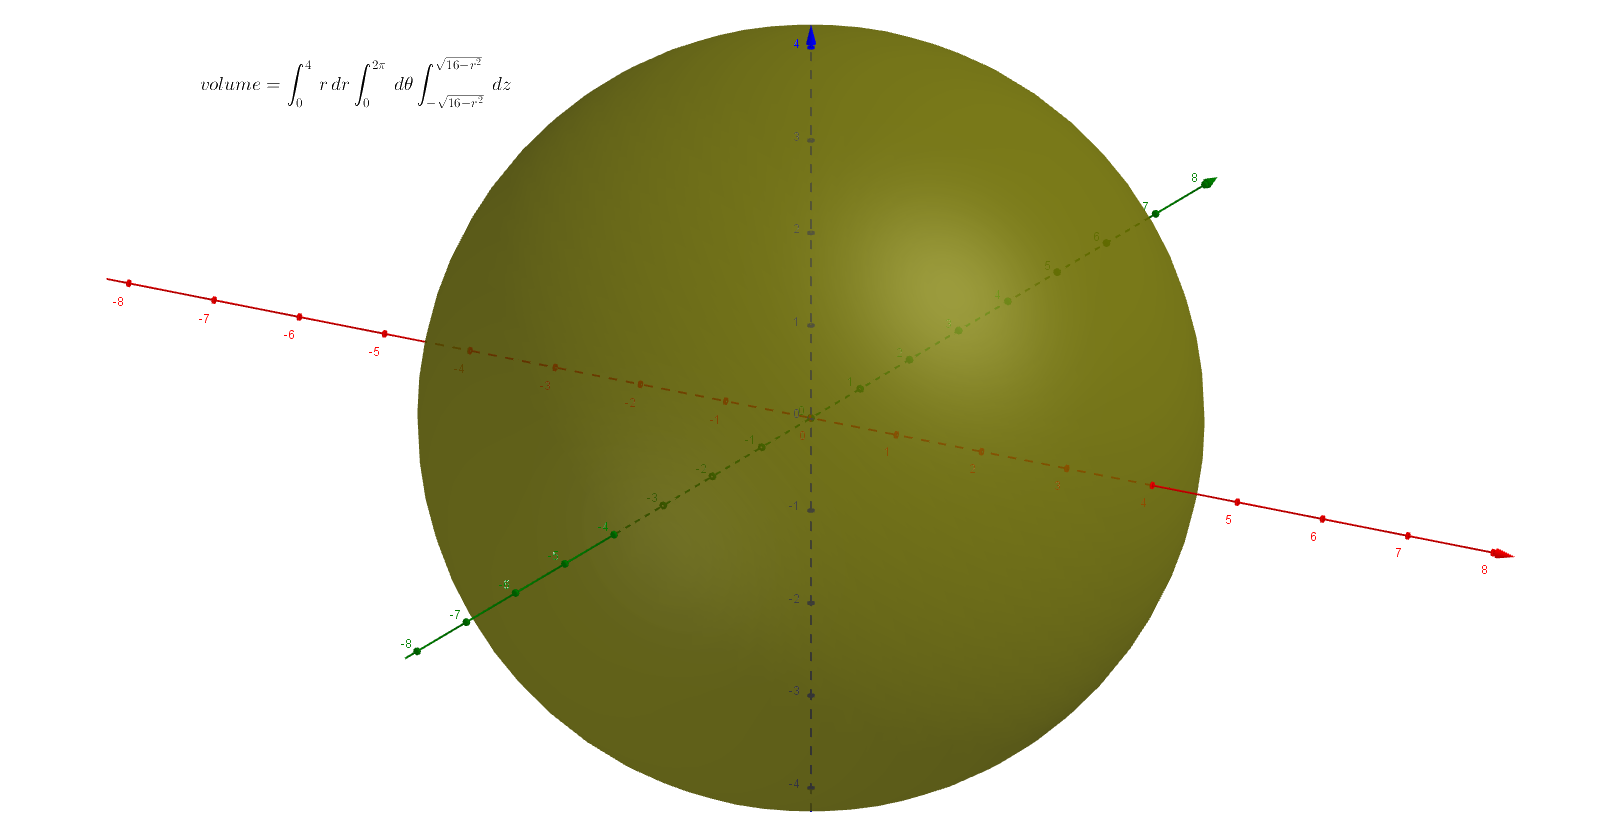
\includegraphics[width=0.5\textwidth]{v28_a04_e01.png}		
	\end{figure}
	
	\begin{gather*}
		x^2 + y^2 + z^2 = 16 \Rightarrow z^2 = 16 - x^2 - y^2 \Rightarrow z = \pm\sqrt{16 - x^2 - y^2} =\\ \pm\sqrt{16 - \left(x^2 + y^2\right)} = \pm\sqrt{16 - r^2}
	\end{gather*}
	\begin{equation*}
		0 \leq r \leq 4,\, 0 \leq \theta \leq 2\pi,\, -\sqrt{16 - r^2} \leq z \leq \sqrt{16 - r^2}
	\end{equation*}
	\begin{gather*}
		\int_0^4 \int_0^{2\pi} \int_{-\sqrt{16 - r^2}}^{\sqrt{16 - r^2}} r\, dz d\theta dr = \int_0^4 r\, dr \int_0^{2\pi} d\theta \int_{-\sqrt{16 - r^2}}^{\sqrt{16 - r^2}} dz =\\ \int_0^4 r\, dr \int_0^{2\pi} d\theta \left[z\right]_{-\sqrt{16 - r^2}}^{\sqrt{16 - r^2}} = \int_0^4 r\, dr \int_0^{2\pi} d\theta \left[\sqrt{16 - r^2} + \sqrt{16 - r^2}\right] =\\ \int_0^4 r\, dr \int_0^{2\pi} d\theta \left[2\sqrt{16 - r^2}\right] = 2\int_0^4 \sqrt{16 - r^2}\,r\, dr \int_0^{2\pi} d\theta =\\ {\overstrike{2}}\int_0^4 \sqrt{u}\left(\dfrac{-du}{\overstrike{2}}\right) \left[\theta\right]_0^{2\pi} = -2\pi\int_0^4 u^{\frac{1}{2}}\, du = -2\pi \left[\dfrac{u^{\frac{3}{2}}}{\left(\dfrac{3}{2}\right)}\right]_0^4 = -2\pi\left[\dfrac{2\sqrt{u^3}}{3}\right]_0^4 =\\ \dfrac{-4\pi}{3}\left[\sqrt{\left(16 - r^2\right)^3}\right]_0^4 = \dfrac{-4\pi}{3}\left[\overstrike{\sqrt{\left(16 - 4^2\right)^3}} - \sqrt{\left(16 - 0^2\right)^3}\right] = \dfrac{-4\pi}{3}\left(-\sqrt{\left(4^2\right)^3}\right) =\\ \dfrac{-4\pi}{3}\left(-4^3\right) = \dfrac{256\pi}{3}
	\end{gather*}
	\begin{equation*}
		u = 16 - r^2 \Rightarrow \dfrac{-du}{2} = r\, dr
	\end{equation*}
\end{enumerate}